% this TeX file provides an awesome example of how TeX will make super 
% awesome tables, at the cost of your of what happens when you try to make a
% table that is very complicated.
% Originally turned in for Dr. Nico's Security Class
\documentclass[11pt]{article}


% Use wide margins, but not quite so wide as fullpage.sty
\marginparwidth 0.5in 
\oddsidemargin 0.25in 
\evensidemargin 0.25in 
\marginparsep 0.25in
\topmargin 0.25in 
\textwidth 6in \textheight 8 in
% That's about enough definitions

% multirow allows you to combine rows in columns
\usepackage{multirow}
% tabularx allows manual tweaking of column width
\usepackage{tabularx}
% longtable does better format for tables that span pages
\usepackage{longtable}
\usepackage{graphicx}
\begin{document}
% this is an alternate method of creating a title
%\hfill\vbox{\hbox{Gius, Mark}
%       \hbox{Cpe 456, Section 01}  
%       \hbox{Lab 1}    
%       \hbox{\today}}\par
%
%\bigskip
%\centerline{\Large\bf Lab 1: Security Audit}\par
%\bigskip
\author{Daniel Ocampo   }
\title{Lab 6: Political Science Exploratory Data Analysis}
\maketitle

\section{Presentation}
During the lab session next Friday, 20 th of October your group will give a short (5-10
minute) presentation on the first two steps described above. Specifically, your presentation
should discuss the data set you have selected and the types of questions you generated with the
justification for each.
\section{Analysis and Solution Generation}

1. Your Political Science Data Analysis: In addition to the R code that provides your
solutions, you are to write a report that includes the following:\\
\section{Part A}

(a) A brief explanation of the data and its headers. Remember to review the article’s
Research Methods and Results sections.\\

The columns that are in the data are simple the first one is the name of all of the states from the United States. The second column has the state number which is not really necessary in my opinion it is somewhat like a counter. GSP Gross state product, which pretty much a measure of the state output. The next column that we have is the population, The reason we have this is to what is the population within the people. Also note that the population size is the same for every state in terms of year because does not get updated during that time frame. The population might in the sense that it is correlated to ideology, so For example the government ideology might be  a little more liberal but nearly half of the population might Conservative. In California for Example, it is very liberal but they still have a fair share of conservatives. We also a columns on the citizen Ideology, which usually similar to the government ideology. \\


\section{Part B}
(b) Five (5) questions about your data set. Also, justify your selection of these particular questions (how asking these questions maybe helpful).\\




\begin{enumerate}
\item Which states have the largest discrepancy between government and citizen ideologies?\\
This  question can tell us how much of difference there is when government and citizen Ideology. In the sense of how much different they are between each other. The data is very interesting because I would assume the number would be very low, but it turns out that there is great discrepancy between much of the states. 




\item Which states have had the largest shift between government and citizen ideologies?
We can see that their is quite a few shift between government and citizen ideologies. there a few states where not much of difference between them but there are some that are very different. 



\item What is the correlation between poverty rates and government ideologies?

There is no real correlation between poverty rate and government ideology. The data fluctuate to much for there to be a difference.  


\item If there is a correlation, does it differ if citizen ideologies are used instead?

Again there was no correlation, between the two, there were to many changing factors between the data. 

\end{enumerate}

\section{Part C}
(c) The answers to your five questions including any appropriate transformations and visualizations that were produced during research.\\
\begin{figure}[ht!]
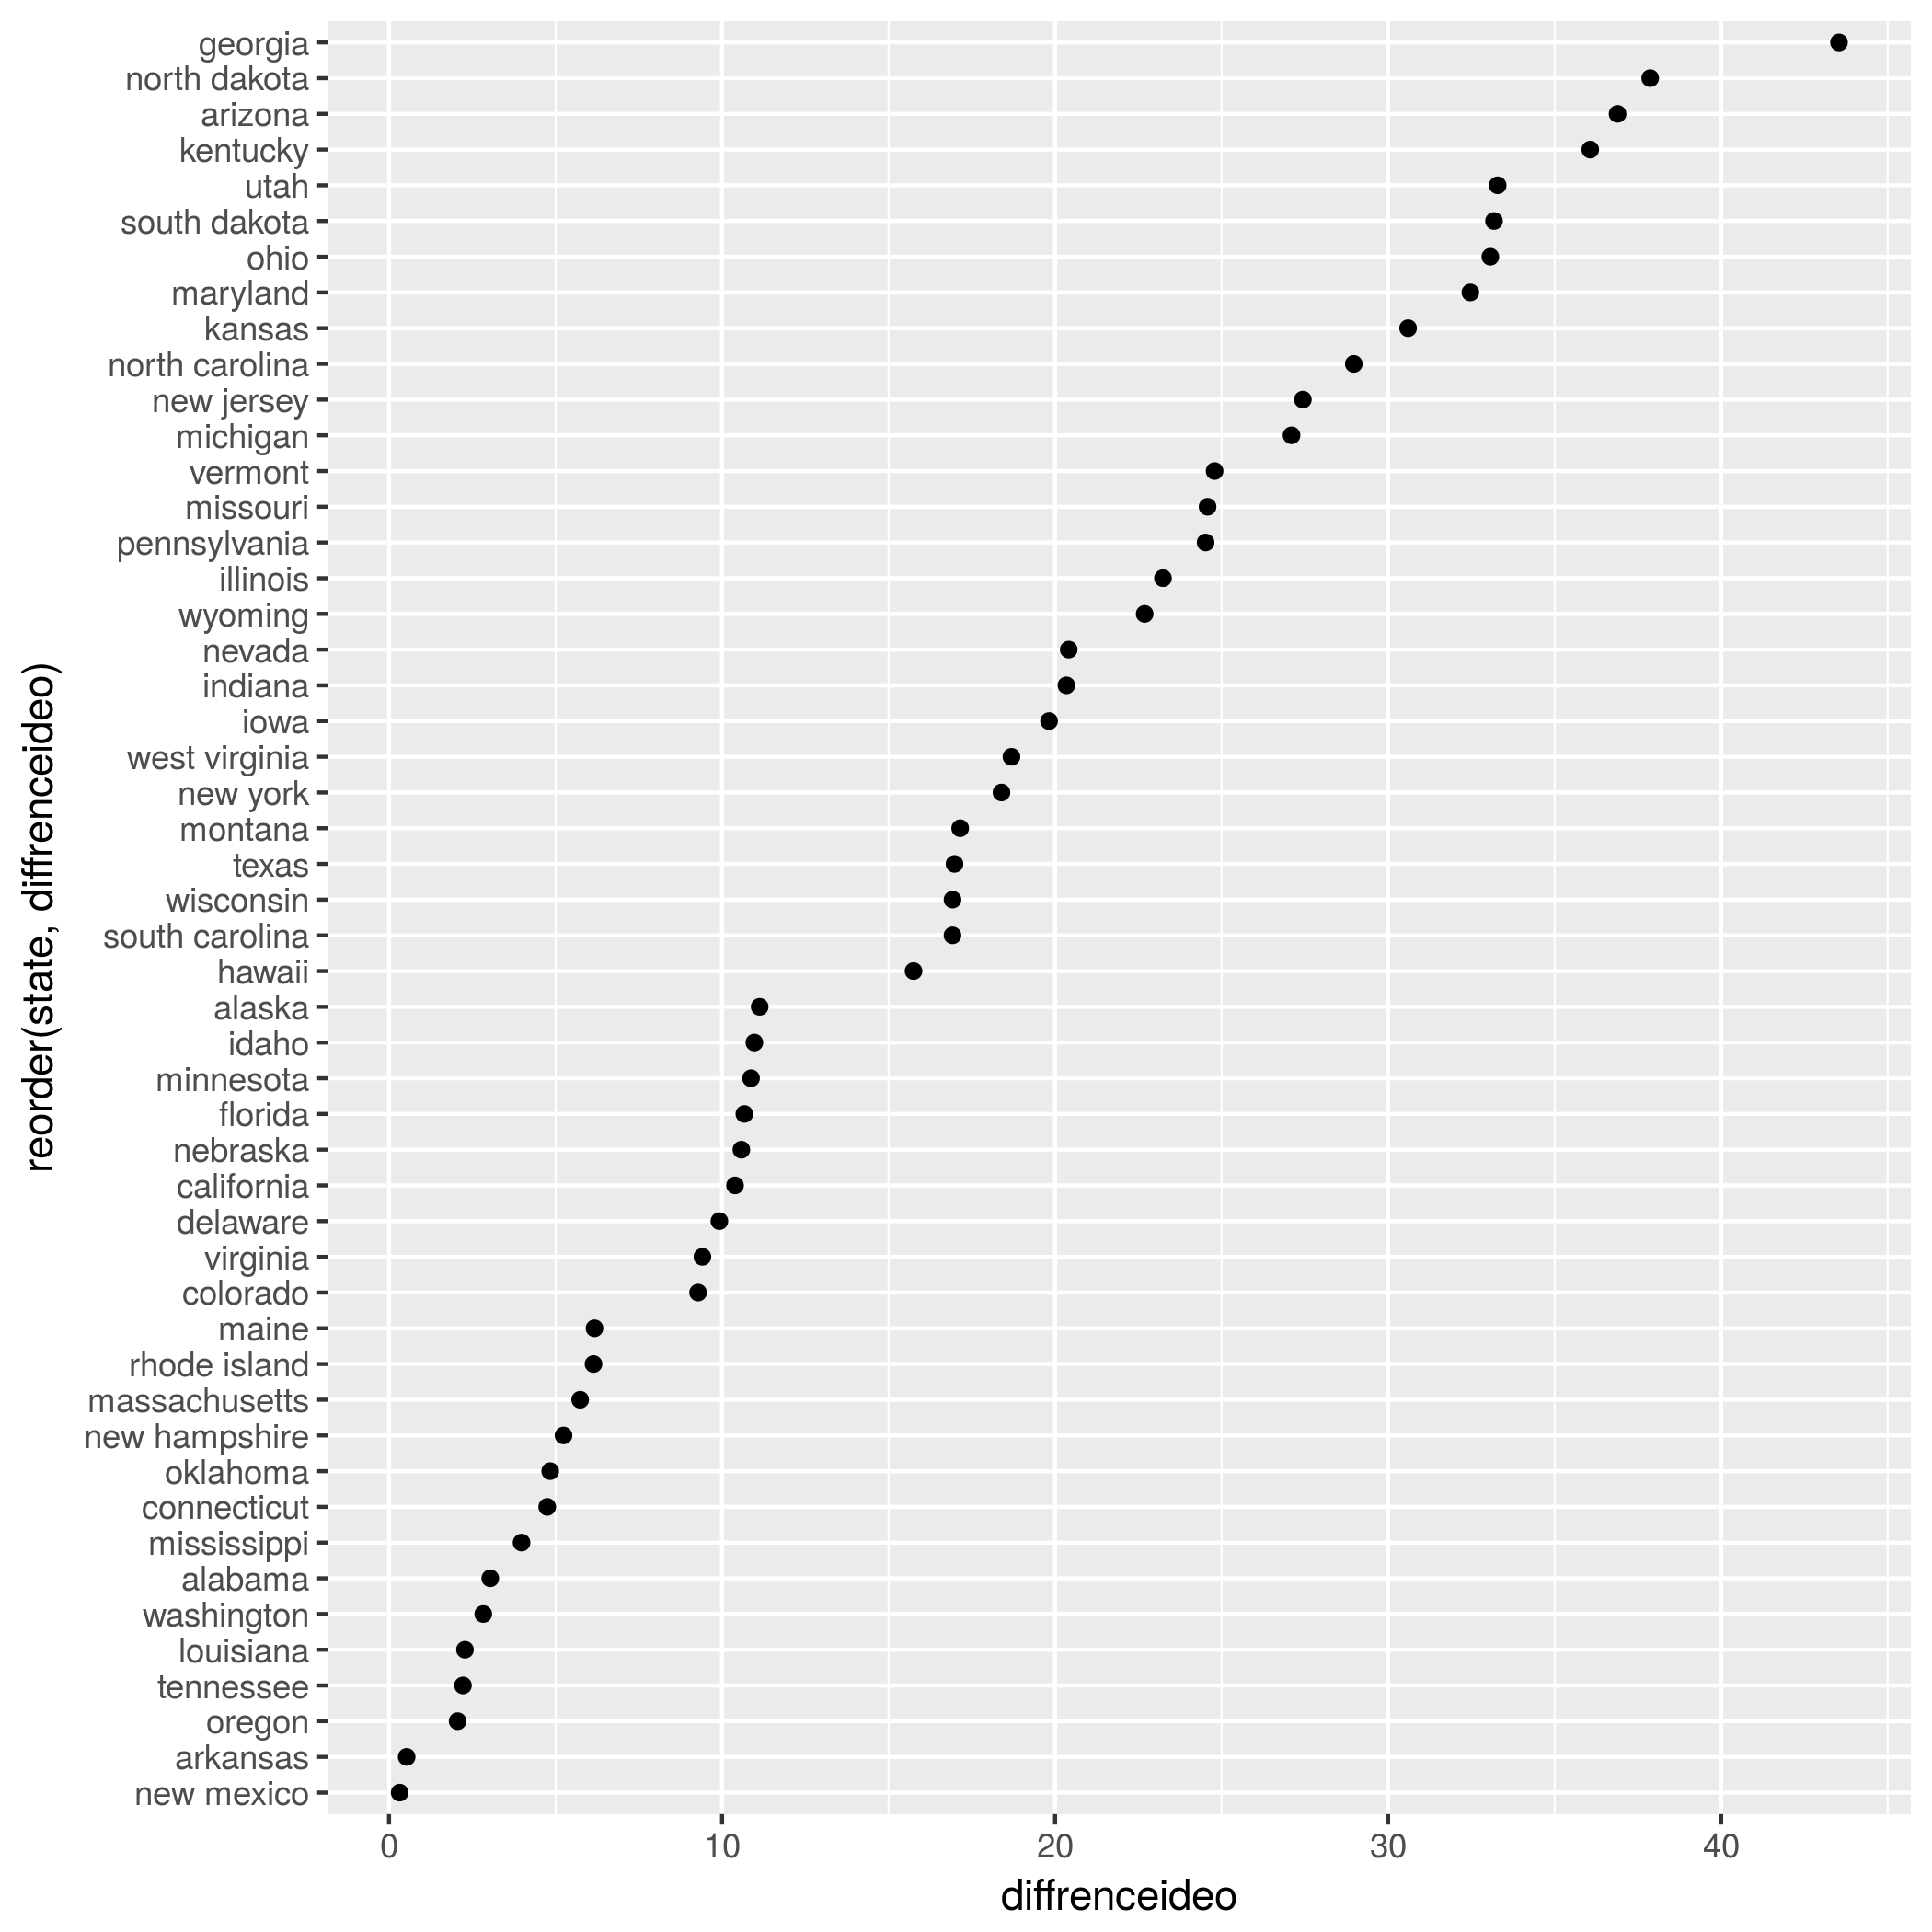
\includegraphics[scale = .5]{graph1.png}
\centering
\end{figure}

\begin{figure}[ht!]
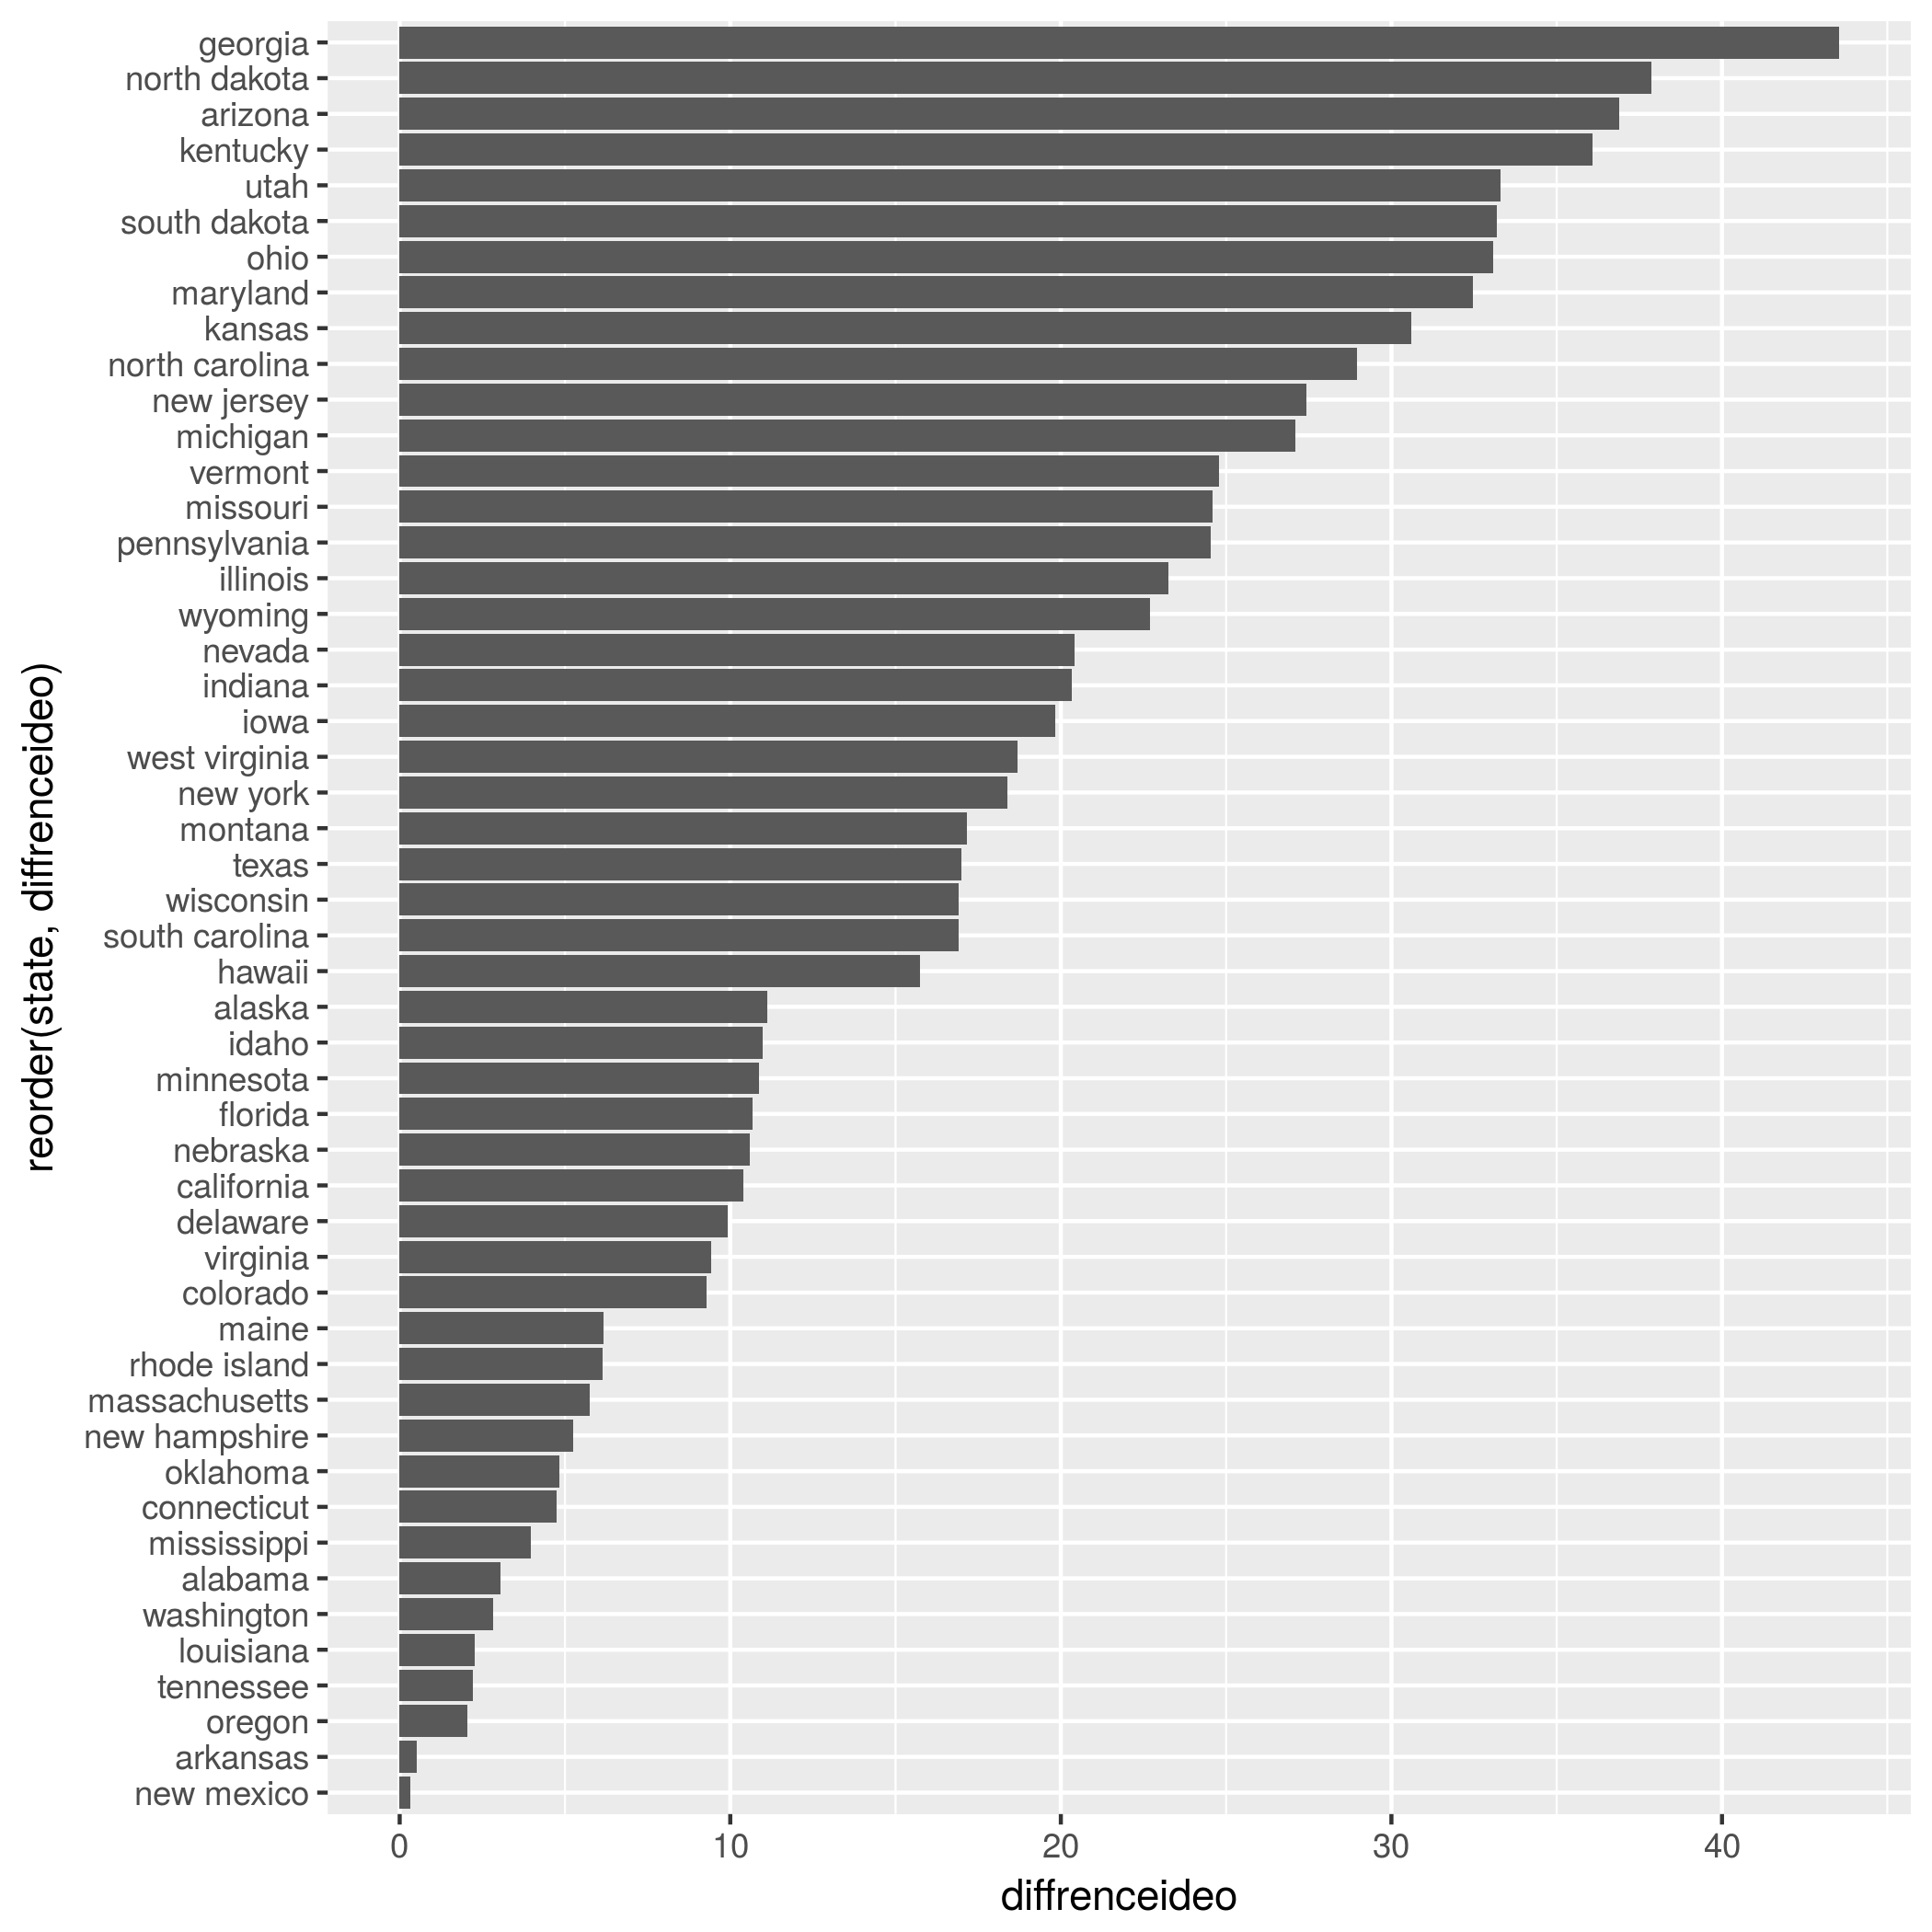
\includegraphics[scale = .5]{graph2.png}
\centering
\end{figure}

\begin{figure}[ht!]
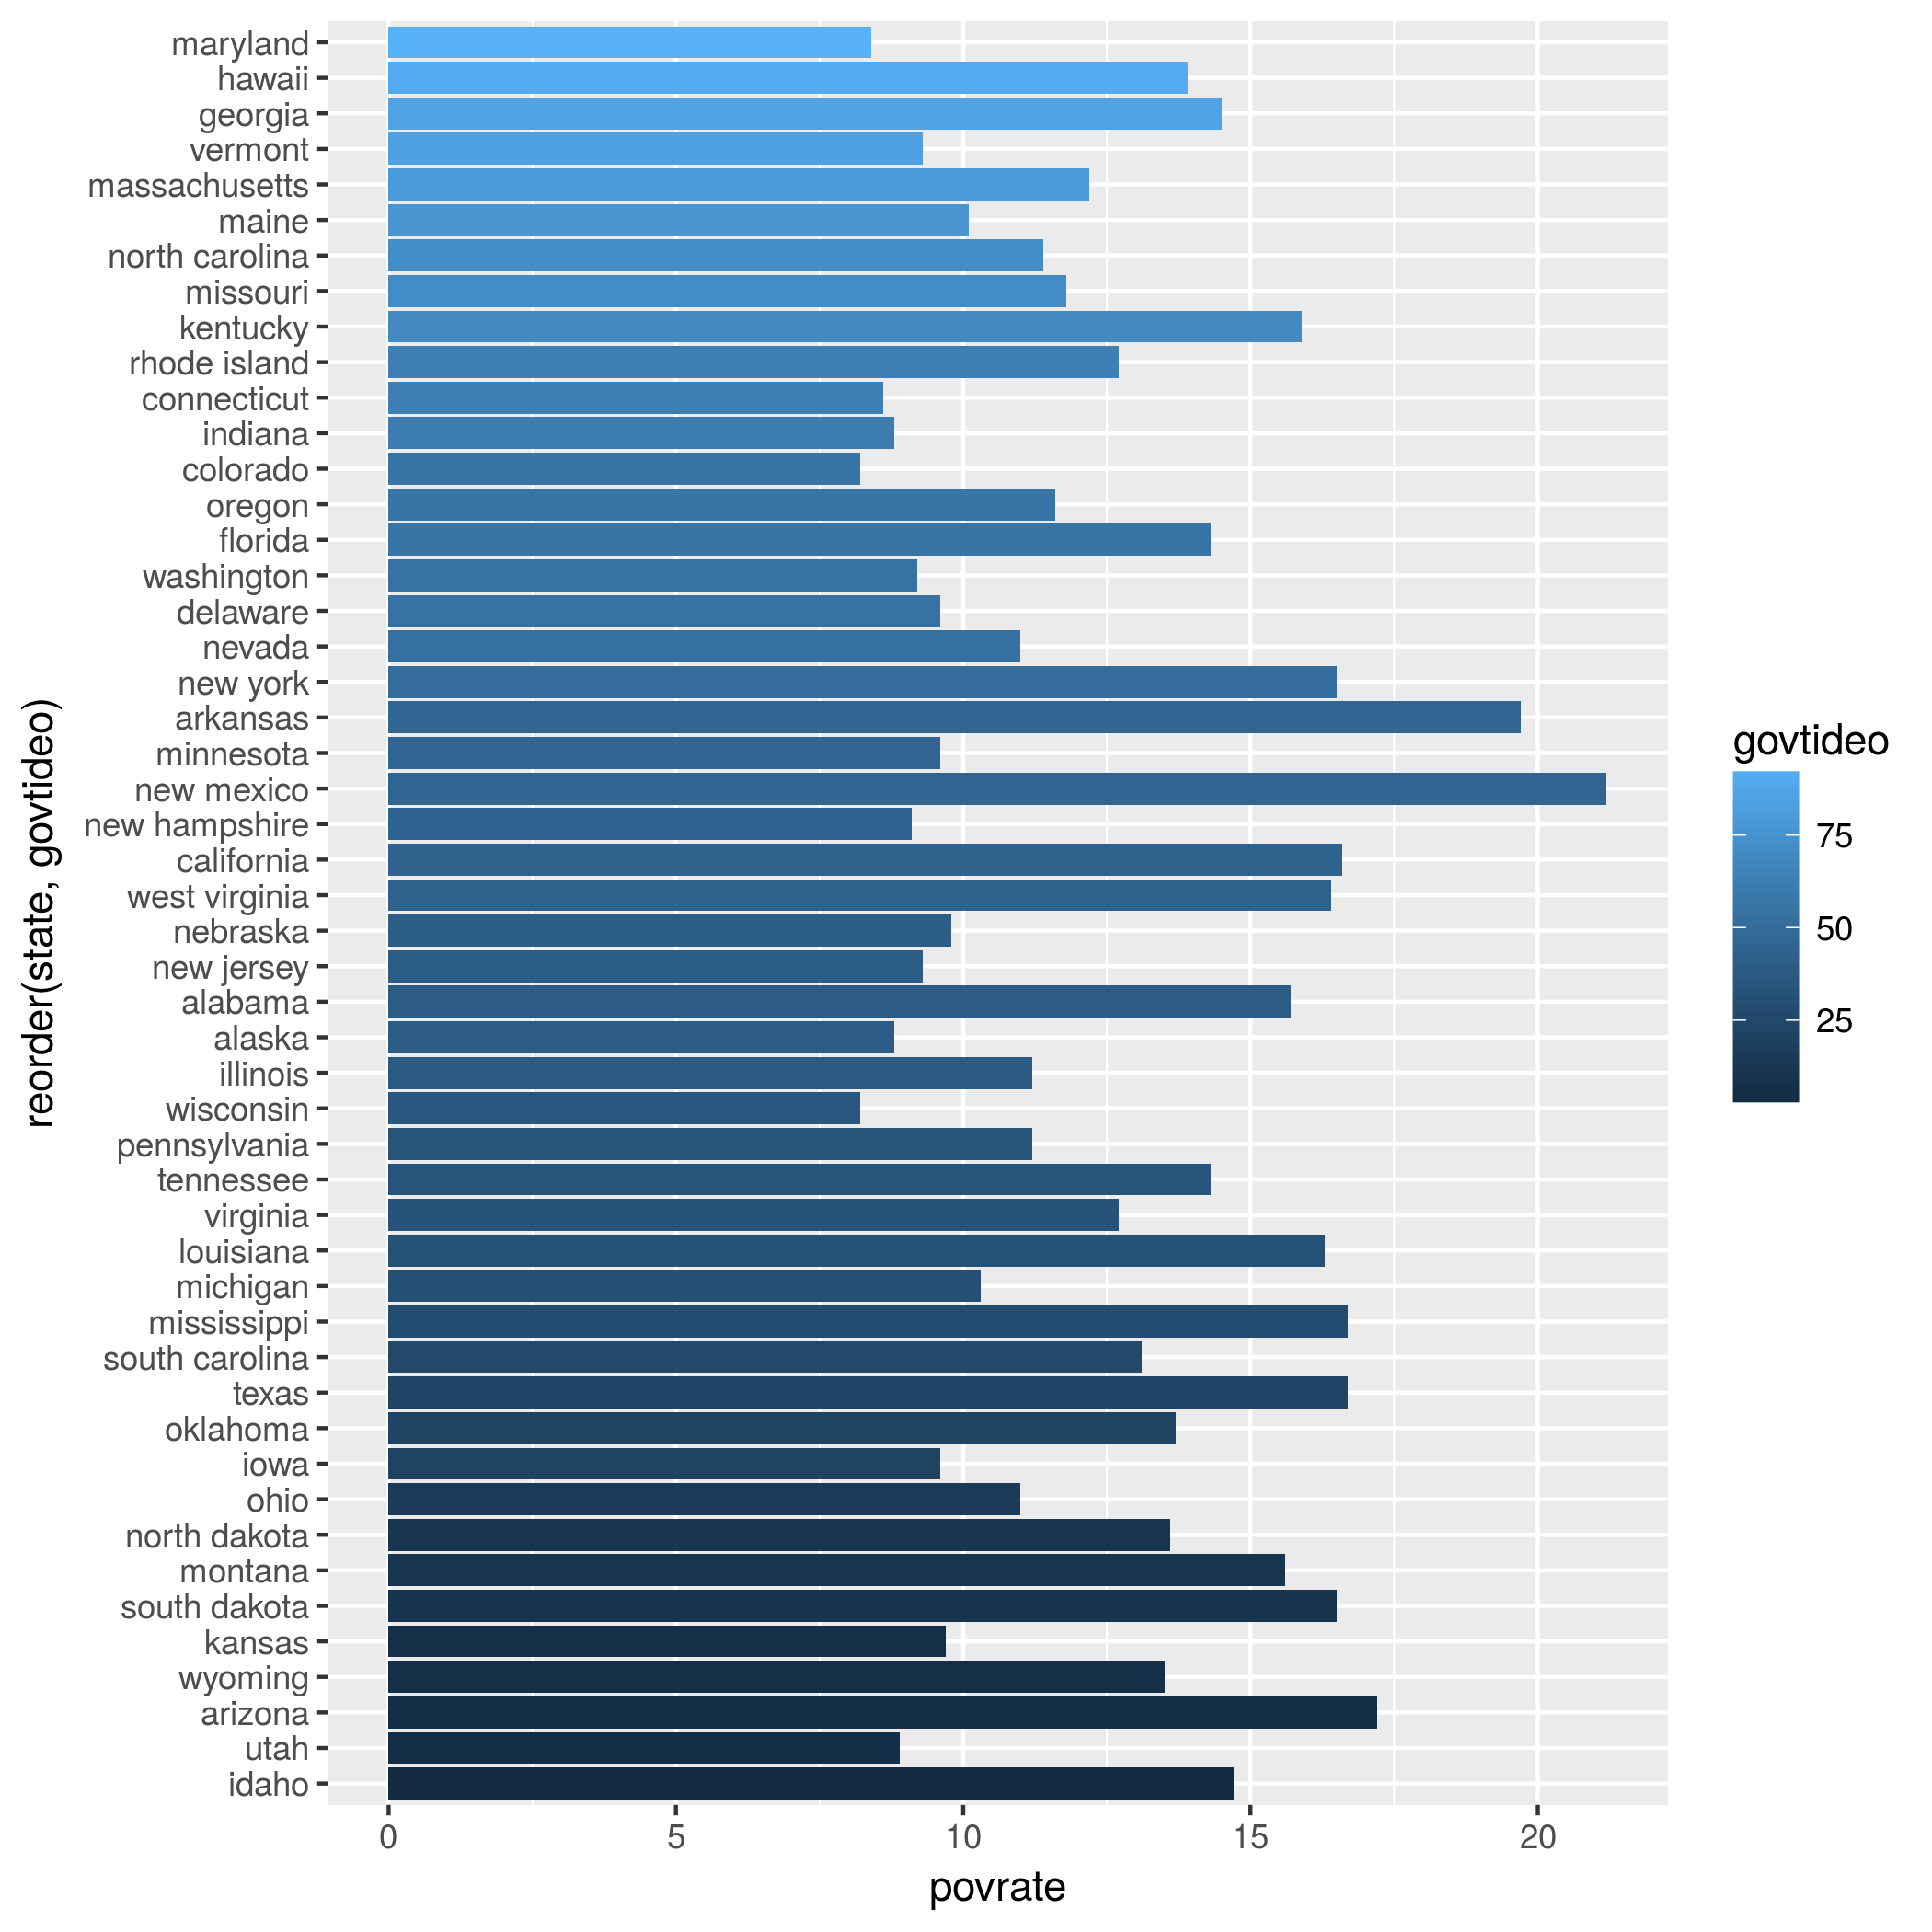
\includegraphics[scale = .5]{graph3.png}
\centering
\end{figure}

\begin{figure}[ht!]
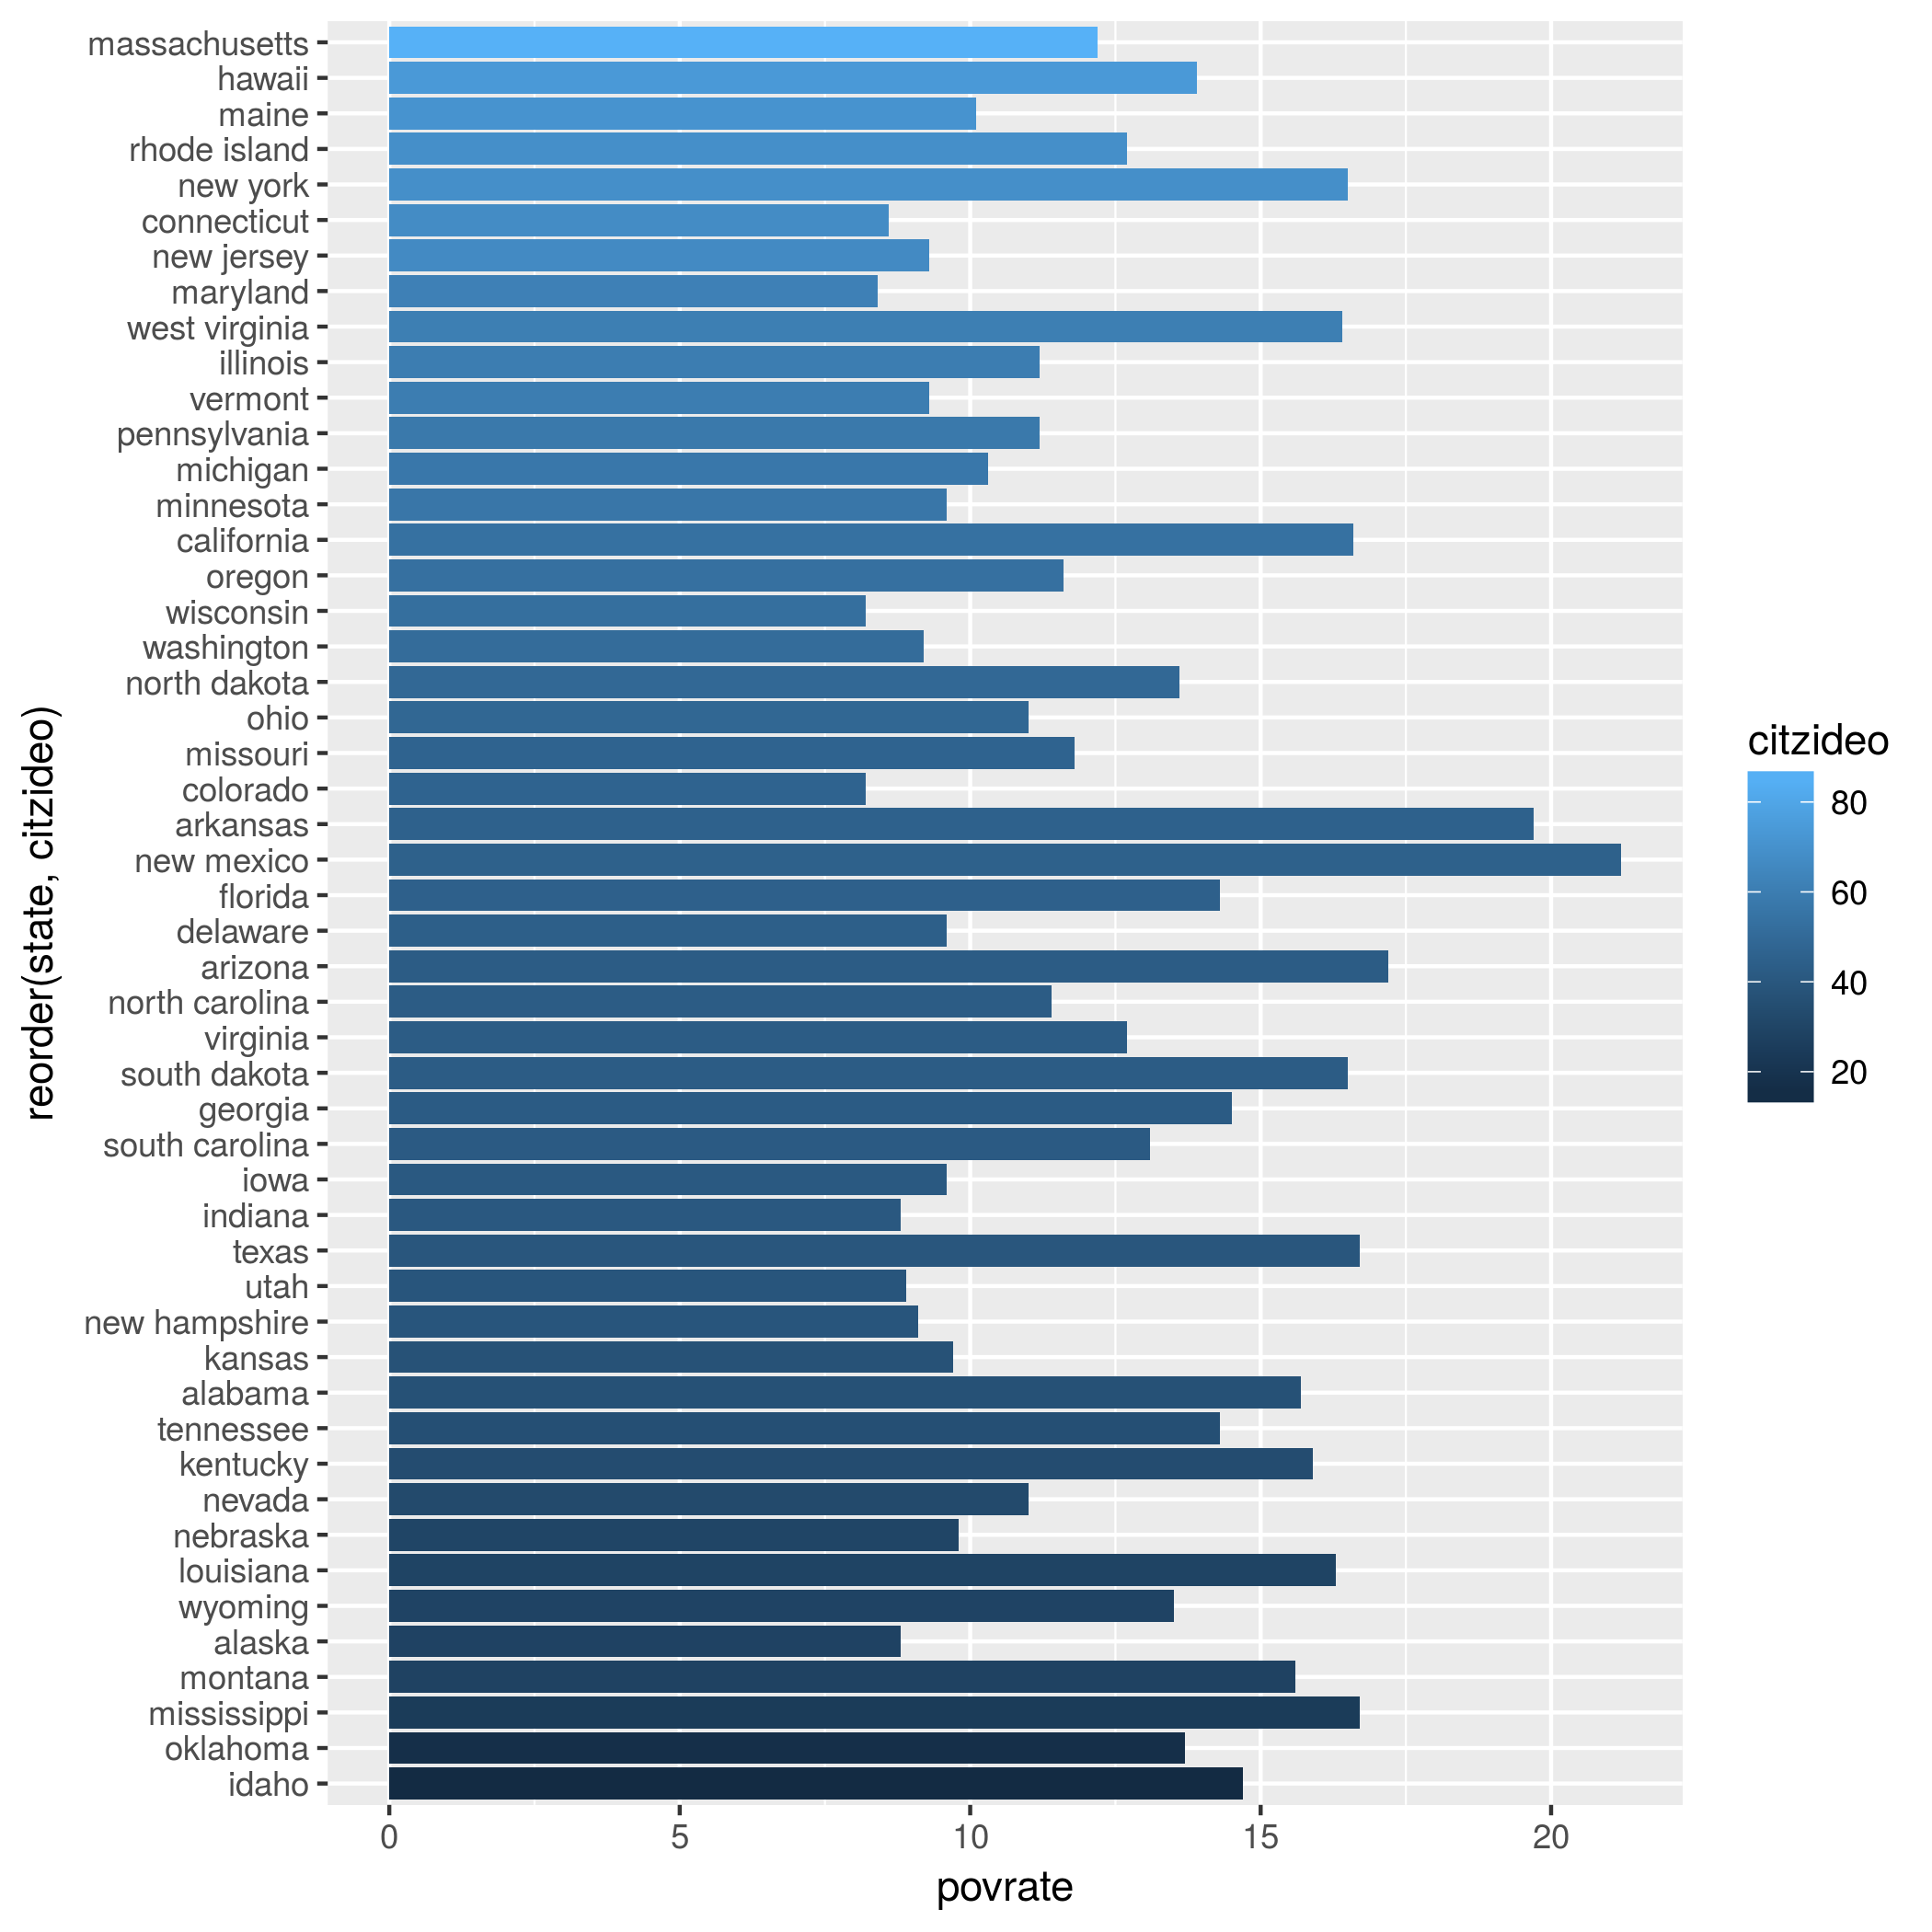
\includegraphics[scale = .5]{graph4.png}
\centering
\end{figure}



\section{Part D}
(d) Your final analysis including your input on modifying your original questions and generating new questions if relevant.\\

There was nothing interesting to me other than fact that I was not expecting it to be so different. Some conservative state had low poverty rate, some liberal states had low poverty rate. I guess everything depends on certain factors, like natural resources maybe, or maybe even maybe ways fiscal policy might effect market. While also taking to consideration monetary policy.


\section{ Dr. Harward} 

(a) Based on Dr. Harward’s provided data and article, discuss the processes to make political
decisions to fund states’ legal services. In addition, discuss how such decisions are
affected. Reflect on potential faults in this system (as you understand them) and how data analysis may be able to identify such faults.
 
 
 I Do not think this enough Data to make any conclusions, her data set is way to small. the population size is different. Also in terms of years it is very difficult to decide things because there are some many other factors. In the sense that we need to take to account of occurring events like the tech bubble, the financial crisis of 2008. The wold trade center, therefore it is very difficulty to look at this data and decide what it means. 




% defines a table that spans pages with columns defined by the sizes seen here
% see http://en.wikibooks.org/wiki/LaTeX/Tables for more information, especially
% sections on spanning and resizing tables

\end{document}
